\chapter{Кватернионы и повороты в пространстве}\label{chap:c24}\markright{Глава 51}
\section{Четыре координаты и новые правила умножения}
\par\addvspace{5pt}\begin{lrbox}{\CatFlowBox}\begin{minipage}[t]{\linewidth}
\setlength{\parskip}{5pt}\setlength{\columnsep}{4.5mm}\setlength{\intextsep}{0pt}
\begin{wrapfigure}[11]{r}{54mm}

\includegraphics[width=54mm,height=58mm,keepaspectratio]{images/unique/art-85.png}
\end{wrapfigure}
Комплексное число описывает пару действительных координат. Следующий пример расширения содержит четыре координаты: одну действительную и три мнимые. Он полезен для знакомства с некоммутативной алгеброй и для описания поворотов в трёхмерном пространстве. Эта дополнительная глава опирается на комплексные числа и матрицы; для начала математического анализа её можно отложить.
\par\WFclear\end{minipage}\end{lrbox}%
\ifdim\dimexpr\ht\CatFlowBox+\dp\CatFlowBox\relax<64mm\dp\CatFlowBox=\dimexpr64mm-\ht\CatFlowBox\relax\fi%
\noindent\usebox{\CatFlowBox}\par\addvspace{5pt}
\begin{definition}
\term{Кватернионы} (\emph{quaternions}) — множество \(\mathbb H=\mathbb C\times\mathbb C\) с покоординатным сложением; умножение задаётся формулой
\[
(a,b)(c,d)=(ac-b\overline d,\;ad+b\overline c).
\]
Здесь \(a,b,c,d\in\mathbb C\), а черта означает комплексное сопряжение. Действительное число \(t\) отождествляется с \((t,0)\).
\end{definition}
Положим \(1=(1,0)\), \(i=(i_{\mathbb C},0)\), \(j=(0,1)\), \(k=(0,i_{\mathbb C})\). Поэтому пара \((x_0+x_1i_{\mathbb C},x_2+x_3i_{\mathbb C})\) записывается единственным образом как \(q=x_0+x_1i+x_2j+x_3k\), где все \(x_r\) действительны. Значок \(i_{\mathbb C}\) нужен только при построении: дальше \(i\) обозначает тот же комплексный элемент внутри \(\mathbb H\).

\begin{center}\renewcommand{\arraystretch}{1.25}
\begin{tabular}{c|rrrr}
\(\cdot\)&\(1\)&\(i\)&\(j\)&\(k\)\\\hline
\(1\)&\(1\)&\(i\)&\(j\)&\(k\)\\
\(i\)&\(i\)&\(-1\)&\(k\)&\(-j\)\\
\(j\)&\(j\)&\(-k\)&\(-1\)&\(i\)\\
\(k\)&\(k\)&\(j\)&\(-i\)&\(-1\)
\end{tabular}\end{center}
В таблице первый множитель выбирается по строке, второй — по столбцу. Например, \(ij=k\), но \(ji=-k\). Произведение общих кватернионов раскрывается по дистрибутивности, сохраняя порядок множителей. Уже эта таблица показывает, почему запись дроби с кватернионным знаменателем без уточнения стороны была бы неоднозначной.

\begin{theorem}[Ассоциативность кватернионного умножения]\label{thm:legacy-c24-1}
Для любых \(p,q,r\in\mathbb H\) выполнено \((pq)r=p(qr)\). Сложение коммутативно и ассоциативно; умножение дистрибутивно относительно сложения с обеих сторон и имеет единицу \(1\).
\end{theorem}
\begin{proof}
Поставим паре \((a,b)\) в соответствие комплексную матрицу
\[
M(a,b)=\begin{pmatrix}a&b\\-\overline b&\overline a\end{pmatrix}.
\]
Непосредственное умножение даёт \(M(a,b)M(c,d)=M(ac-b\overline d,ad+b\overline c)\). Отображение \(M\) инъективно: пара восстанавливается по первой строке. Ассоциативность матриц поэтому даёт \(M((pq)r)=M(p(qr))\), а значит, равенство кватернионов. Остальные свойства следуют покоординатно из определения; в частности, умножение любой пары на \((1,0)\) с каждой стороны возвращает эту пару.
\end{proof}

\section{Сопряжение, норма и деление}
\begin{definition}
\term{Сопряжение кватерниона} (\emph{quaternion conjugation}) задаётся формулой \(\overline q=x_0-x_1i-x_2j-x_3k\); для пары это \(\overline{(a,b)}=(\overline a,-b)\).
\end{definition}
\begin{definition}
\term{Норма кватерниона} (\emph{quaternion norm}) — число \(|q|=\sqrt{x_0^2+x_1^2+x_2^2+x_3^2}\). Обозначим \(N(q)=|q|^2\); это квадрат нормы, а не сама норма.
\end{definition}
\begin{definition}
\term{Действительная часть} (\emph{real part}) — \(\operatorname{Re}q=x_0\).
\end{definition}
\begin{theorem}[Сопряжение и норма]\label{thm:legacy-c24-2}
Для \(p,q\in\mathbb H\) выполнены
\[
\overline{pq}=\overline q\,\overline p,\qquad
q\overline q=\overline q q=N(q),\qquad N(pq)=N(p)N(q).
\]
При \(q\ne0\) существует двусторонний обратный \(q^{-1}=\frac{\overline q}{N(q)}\).
\end{theorem}
\begin{proof}
Для пары \(q=(a,b)\) умножение на \((\overline a,-b)\) с любой стороны даёт \((|a|^2+|b|^2,0)\). Кроме того, матрица \(M(\overline q)\) получается из \(M(q)\) транспонированием и сопряжением каждого элемента. Такое действие обращает порядок произведения матриц: это проверяется по формуле для их элементов. Инъективность \(M\) доказывает первое равенство. Теперь, пользуясь уже доказанной ассоциативностью, получаем
\[
(pq)\overline{pq}=p(q\overline q)\overline p=N(q)p\overline p=N(p)N(q).
\]
При \(q\ne0\) сумма квадратов его координат положительна, поэтому деление на действительное \(N(q)\) допустимо и даёт обратный с обеих сторон.
\end{proof}
\begin{definition}
\term{Тело} (\emph{division ring; skew field}) — ассоциативное кольцо с \(1\ne0\), в котором каждый ненулевой элемент имеет двусторонний обратный. Коммутативность умножения не требуется. Таким образом, \(\mathbb H\) — тело, но не поле.
\end{definition}
Чтобы решить \(qx=b\) при \(q\ne0\), умножаем слева и получаем \(x=q^{-1}b\). Для \(xq=b\) ответ иной: \(x=bq^{-1}\). Здесь сокращение обосновано и обратимостью, и ассоциативностью. Порядок в формуле для сопряжения произведения тоже существенен: его нельзя копировать из комплексного случая без изменения.

\begin{theorem}[Два полезных равенства]\label{thm:legacy-c24-3}
Для \(u,v\in\mathbb H\) выполнены
\[
\operatorname{Re}(uv)=\operatorname{Re}(vu),\qquad
N(u+v)=N(u)+N(v)+2\operatorname{Re}(u\overline v).
\]
\end{theorem}
\begin{proof}
Если координаты \(u\) равны \(u_0,\ldots,u_3\), а координаты \(v\) — \(v_0,\ldots,v_3\), то таблица умножения даёт \(\operatorname{Re}(uv)=u_0v_0-u_1v_1-u_2v_2-u_3v_3\). Выражение симметрично. Во второй формуле \(\operatorname{Re}(u\overline v)=\sum_{r=0}^3u_rv_r\), а раскрытие \(\sum_{r=0}^3(u_r+v_r)^2\) даёт требуемое равенство.
\end{proof}

\section{Как описать поворот}
\begin{definition}
\term{Чисто мнимый кватернион} (\emph{pure imaginary quaternion}) имеет нулевую действительную часть: \(v=xi+yj+zk\). Его можно отождествить с вектором \((x,y,z)\in\mathbb R^3\).
\end{definition}
\begin{definition}
\term{Единичный кватернион} (\emph{unit quaternion}) удовлетворяет \(|q|=1\).
\end{definition}
\par\addvspace{5pt}\begin{lrbox}{\CatFlowBox}\begin{minipage}[t]{\linewidth}
\setlength{\parskip}{5pt}\setlength{\columnsep}{4.5mm}\setlength{\intextsep}{0pt}
\begin{wrapfigure}[9]{l}{54mm}

\includegraphics[width=54mm,height=58mm,keepaspectratio]{images/unique/art-86.png}
\end{wrapfigure}
Трёхмерный вектор становится частью алгебры, в которой удобно вычислять повороты. Для единичного \(q\) рассмотрим \(T_q(v)=qv\overline q\). В отличие от плоской формулы \(z\mapsto wz\), здесь участвуют два умножения, с разных сторон. Такая запись используется в компьютерной графике и управлении ориентацией: последовательность преобразований можно вычислять умножением кватернионов.
\par\WFclear\end{minipage}\end{lrbox}%
\ifdim\dimexpr\ht\CatFlowBox+\dp\CatFlowBox\relax<64mm\dp\CatFlowBox=\dimexpr64mm-\ht\CatFlowBox\relax\fi%
\noindent\usebox{\CatFlowBox}\par\addvspace{5pt}
\begin{theorem}[Сохранение длин и поворот вокруг оси]\label{thm:legacy-c24-4}
Для единичного \(q\) отображение \(T_q\) линейно над \(\mathbb R\), переводит чисто мнимые кватернионы в чисто мнимые и сохраняет их нормы. Если
\[
q=\cos\frac\theta2+k\sin\frac\theta2,
\]
то \(T_q(xi+yj+zk)=(x\cos\theta-y\sin\theta)i+(x\sin\theta+y\cos\theta)j+zk\).
\end{theorem}
\begin{proof}
Линейность следует из дистрибутивности и умножения на действительные числа. Так как \(\overline v=-v\), имеем \(\overline{qv\overline q}=q\overline v\,\overline q=-qv\overline q\), то есть результат чисто мнимый. Мультипликативность нормы даёт \(|qv\overline q|=|q|\,|v|\,|\overline q|=|v|\). Положим \(c=\cos\frac\theta2\), \(s=\sin\frac\theta2\). По таблице
\[
(c+ks)i(c-ks)=(c^2-s^2)i+2csj,
\]
\[
(c+ks)j(c-ks)=-2csi+(c^2-s^2)j,
\]
а \((c+ks)k(c-ks)=k\). Формулы двойного угла и линейность завершают доказательство.
\end{proof}
Два кватерниона \(q\) и \(-q\) задают одно преобразование, поскольку два знака минус сокращаются. Например, \(q=\frac{1+k}{\sqrt2}\) задаёт поворот на \(\frac\pi2\): ось \(x\) переходит в ось \(y\), ось \(y\) — в противоположное направление оси \(x\), а ось \(z\) остаётся на месте. Направления задаются правой системой координат, как в выведенной формуле.

\Needspace{7\baselineskip}\section*{Задачи}
\begingroup\setlength{\parskip}{2pt}
\noindent\begin{minipage}[t]{\linewidth}\textbf{51.1.} Вычисли \(ij,ji,jk,kj,ki,ik\). Какие пары дают разные результаты при перестановке?\par\end{minipage}\par
\noindent\begin{minipage}[t]{\linewidth}\textbf{51.2.} Для \(p=1+2i-j\), \(q=3-i+4k\) найди \(p+q\) и \(p-q\).\par\end{minipage}\par
\noindent\begin{minipage}[t]{\linewidth}\textbf{51.3.} Раскрой \((1+i)(1+j)\) и \((1+j)(1+i)\).\par\end{minipage}\par
\noindent\begin{minipage}[t]{\linewidth}\textbf{51.4.} Найди \((i+j)^2\) и объясни, почему здесь нельзя заменить смешанные слагаемые на \(2ij\).\par\end{minipage}\par
\noindent\begin{minipage}[t]{\linewidth}\textbf{51.5.} Для \(q=1+2i-2j+4k\) найди \(\overline q\), \(N(q)\), \(|q|\) и \(q^{-1}\).\par\end{minipage}\par
\par\addvspace{5pt}\begin{lrbox}{\CatFlowBox}\begin{minipage}[t]{\linewidth}
\setlength{\parskip}{5pt}\setlength{\columnsep}{4.5mm}\setlength{\intextsep}{0pt}
\begin{wrapfigure}[11]{r}{54mm}
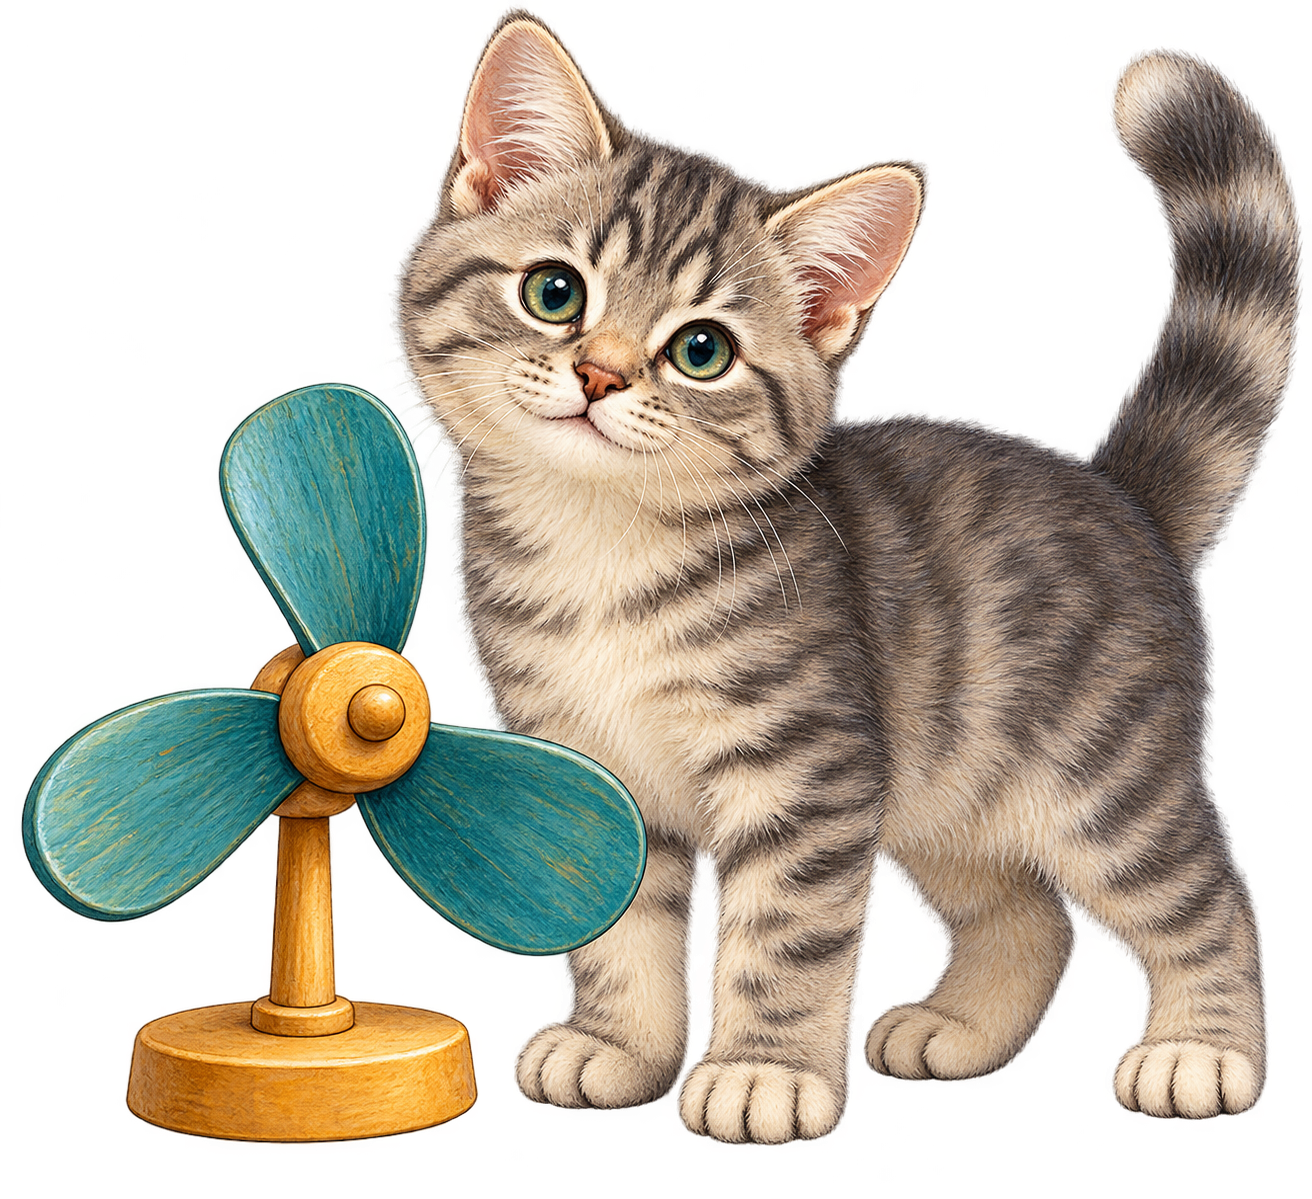
\includegraphics[width=54mm,height=58mm,keepaspectratio]{images/unique/art-87.png}
\end{wrapfigure}
\textbf{51.6.} Реши отдельно \(ix=j\) и \(xi=j\).\par

\textbf{51.7.} Запиши матрицу \(M(q)\) для \(q=1+2i+3j-4k\).\par

\textbf{51.8.} Докажи \(q+\overline q=2\operatorname{Re}q\) и \(\overline{\overline q}=q\).\par

\textbf{51.9.} Докажи, что ненулевые кватернионы не могут иметь нулевое произведение.\par

\textbf{51.10.} Вычисли \((ijk)\), то есть произведение в указанном порядке. Проверь две расстановки скобок.\par

\textbf{51.11.} В графическом редакторе вектор \((2,-1,3)\) поворачивают вокруг оси \(z\) на \(90^\circ\). Используй \(q=\dfrac{1+k}{\sqrt2}\) и найди результат.\par

\textbf{51.12.} Камера должна изменить направление \((1,0,0)\) на \((-1,0,0)\) поворотом вокруг оси \(z\). Подбери единичный кватернион и проверь действие.\par
\par\WFclear\end{minipage}\end{lrbox}%
\ifdim\dimexpr\ht\CatFlowBox+\dp\CatFlowBox\relax<64mm\dp\CatFlowBox=\dimexpr64mm-\ht\CatFlowBox\relax\fi%
\noindent\usebox{\CatFlowBox}\par\addvspace{5pt}

\noindent\begin{minipage}[t]{\linewidth}\textbf{51.13.} Докажи \(T_{-q}(v)=T_q(v)\) для любого единичного \(q\).\par\end{minipage}\par
\noindent\begin{minipage}[t]{\linewidth}\textbf{51.14.}\starmark{} Докажи \(T_p(T_q(v))=T_{pq}(v)\) для единичных \(p,q\). В каком порядке применяются два преобразования?\par\end{minipage}\par
\noindent\begin{minipage}[t]{\linewidth}\textbf{51.15.}\starmark{} Найди все кватернионы \(q\), коммутирующие с \(i\): \(qi=iq\).\par\end{minipage}\par
\noindent\begin{minipage}[t]{\linewidth}\textbf{51.16.}\starmark{} Докажи: если \(q\) коммутирует с каждым кватернионом, то \(q\) является действительным числом.\par\end{minipage}\par
\noindent\begin{minipage}[t]{\linewidth}\textbf{51.17.}\starmark{} Докажи для чисто мнимого \(v=xi+yj+zk\), что \(v^2=-|v|^2\).\par\end{minipage}\par
\noindent\begin{minipage}[t]{\linewidth}\textbf{51.18.}\starmark{} Докажи формулу \((pq)^{-1}=q^{-1}p^{-1}\) при \(p,q\ne0\).\par\end{minipage}\par
\endgroup
